\chapter{Sensing and controlling mirror motion in the radiation pressure eigenbasis} 



\begin{figure}
\begin{centering}
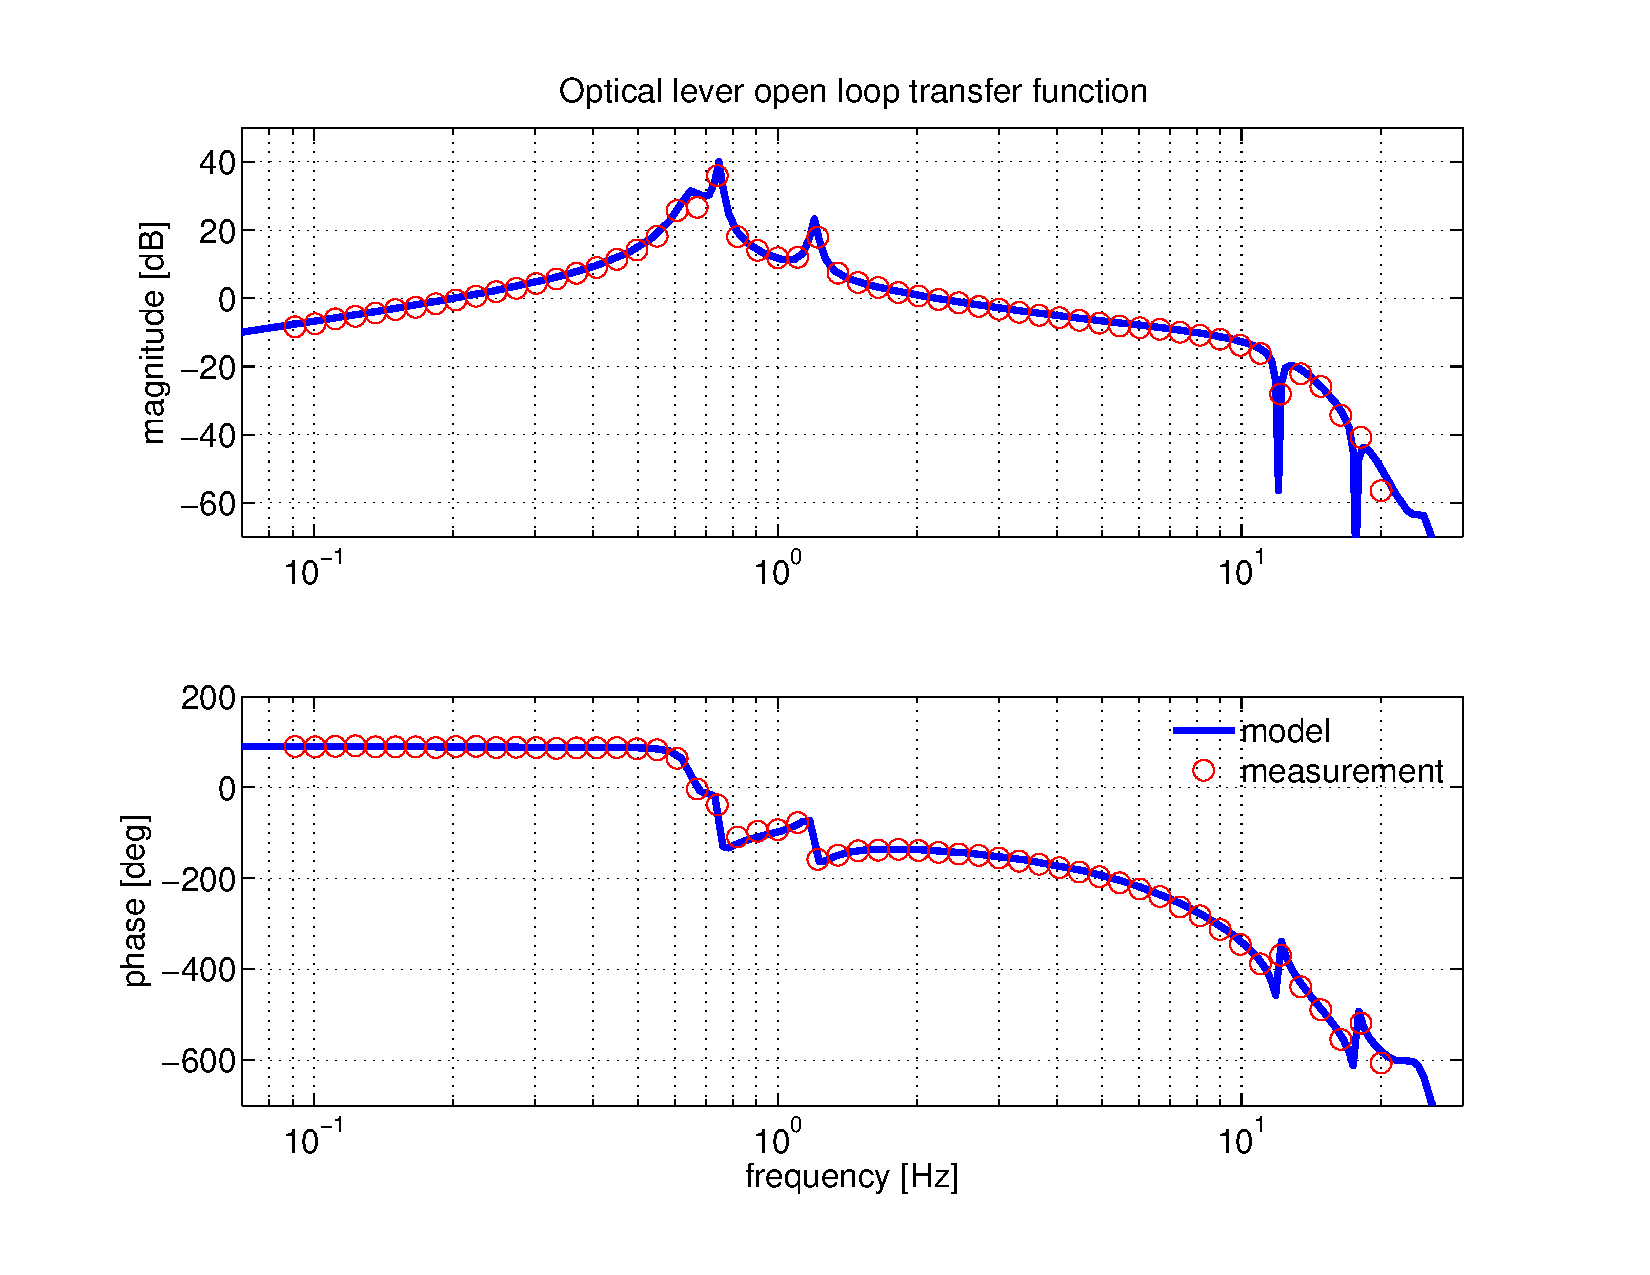
\includegraphics[width=1.0\textwidth]{figures/oplevOLG.pdf}
\caption{ETMX optical lever open loop transfer function. Uses the
  filters in the oplev servo filter bank, only (no coil output
  filters). The model of the plant is tuned to match the data,
  resulting in a pitch resonance of 0.65 Hz and a damping factor of
  $\gamma$ = 0.02. The UGF is at 2.2~Hz and the phase margin is
  $38^\circ$.}
\label{fig:}
\end{centering}
\end{figure}




\section{Introduction}
% The mirror motions must be controlled so that the mirrors are
% stationary with respect to one another as best as possible. The
% mirrors must be held in place at DC, and be quiet at AC. The DC
% pointing is easily determined, but our ability to know exactly how the
% mirrors are moving at AC is limited. The noise floor of the sensors
% dominates the signal above 20 Hz. Therefore, any gain in the servo at
% 20 Hz and above will impress the sensor noise floor onto the mirrors,
% resulting in the introduction of motion rather than suppression. Angle
% to length couplings of the mirror drives make this noise impression
% particularly detrimental since it is comparable to the strain
% sensititivity up to about 70 Hz. In order to avoid having the angular
% control loops be the limiting noise source for DARM up to 70 Hz, a low
% pass filter must be included in the control design. A low pass filter,
% however, changes the phase of the loop such that to maintain loop
% stability, the overall gain must be limited. A compromise must then be
% reached between how much DC gain to use and how much
% noise impression to tolerate. This was achieved for Initial LIGO with
% up to xx~kW circulating power.


The Enhanced LIGO goal of increasing the input power to 30 W from the
Initial LIGO 7 W makes radiation pressure torques cross into the realm
of significance. In particular, the soft opto-mechanical mode which
approached instability for Initial LIGO powers actually becomes
unstable for Enhanced LIGO powers. The static instability requires
high DC gain. The sensors in Initial LIGO, however, were not tuned in
to specifically look for the combined mirror motions that create the
unstable mode. The only way to provide adequate DC control to prevent
the mirrors from falling apart would be to increase the gain of all of
the angular control loops. Since some of the sensors are less good
than others, this would result in extreme impression of noise on
DARM. Thus, to maintain a reasonable noise budget while reigning in
the static instability, we need to make the sensors specifically pick
out the mirror motions that together create this detrimental
mode. This is the basis of the ASC work for Enhanced LIGO--switching
the sensors to the radiation pressure eigenmode basis, and increasing
the gain of the single loop that is sensitive to only the unstable mode. 

In this chapter I show how the angular displacements are sensed and
why control filters implemented in the eigenbasis of radiation
pressure torques is best. 



% \section{Sensing}
% There are five main subsets of sensor systems for the ASC:
% \begin{itemize}
% \item OSEMs
% \item optical levers (MMT3, RM, BS, ITMX, ITMY, ETMX, ETMY) \vspace{-10pt}
% \item camera image (BS)
% \item quadrant photodiodes (QPDX, QPDY) \vspace{-10pt}
% \item wavefront sensors (WFS1, WFS2, WFS3, WFS4) \vspace{-10pt}
% \end{itemize}
% Together, these sensors need to provide enough information to derive
% adequate control signals for 9 mirrors in both pitch and yaw. Both
% absolute motion (AC) and relative motion (DC) need to be
% suppressed. The OSEMs and optical levers provide local AC control to
% the mirrors. The video camera and the QPDs control the pointing of the
% input beam; the video camera works at DC and the QPDs at both DC and
% AC. The WFS provide the top level fine tuning of DC and AC control to
% the 5 main mirrors.


% \subsection{OSEMs}
% The most basic level of control is local damping of each suspended
% optic provided by the OSEMs. This is always on, even when the
% interferometer loses lock. It works by sending current through the
% OSEM coils to keep a constant amount of light on the OSEM shadow
% sensor.


% \subsection{Optical levers}
% The optical levers are local to each large optic and provide a record
% at all times of pitch and yaw pointing of each mirror with respect to
% the ground. The mirrors are velocity-damped only by the optical
% levers; they are not controlled at DC. The optical lever is a HeNe
% laser beam that reflects off of the mirror and onto a QPD. Both the
% laser and QPD are mounted on heavy piers to reduce the seismic noise
% contribution to the QPD signal. The optical lever provides a feedback
% signal to the mirror's coils to reduce the sensed motion. Each large
% optic has its own independent optical lever loop which is almost
% always on, even when the interferometer is out of lock. The optical
% lever loops provide the second level of controlled stabilization of
% the mirrors, after only the local damping.


% \subsection{Camera image}
% The most primitive sensor is that of the physical video camera.  The
% video camera monitors the location of the spot on the beam splitter,
% thus serving as a sensor of the pointing of the input beam. The image
% of the speckle of light reflected off of the beam splitter (see
% Fig. \ref{fig:BCS}) is fed into a labview program which integrates the
% intensity of the image to identify the coordinates of the center of
% the beam spot. This is compared with a hardcoded desired center
% location and a mirror upstream, MMT1 is moved to redirect the input
% beam, minimizing the difference between the desired and actual beam
% spot location on the BS.

% \begin{figure}
% \begin{centering}
% 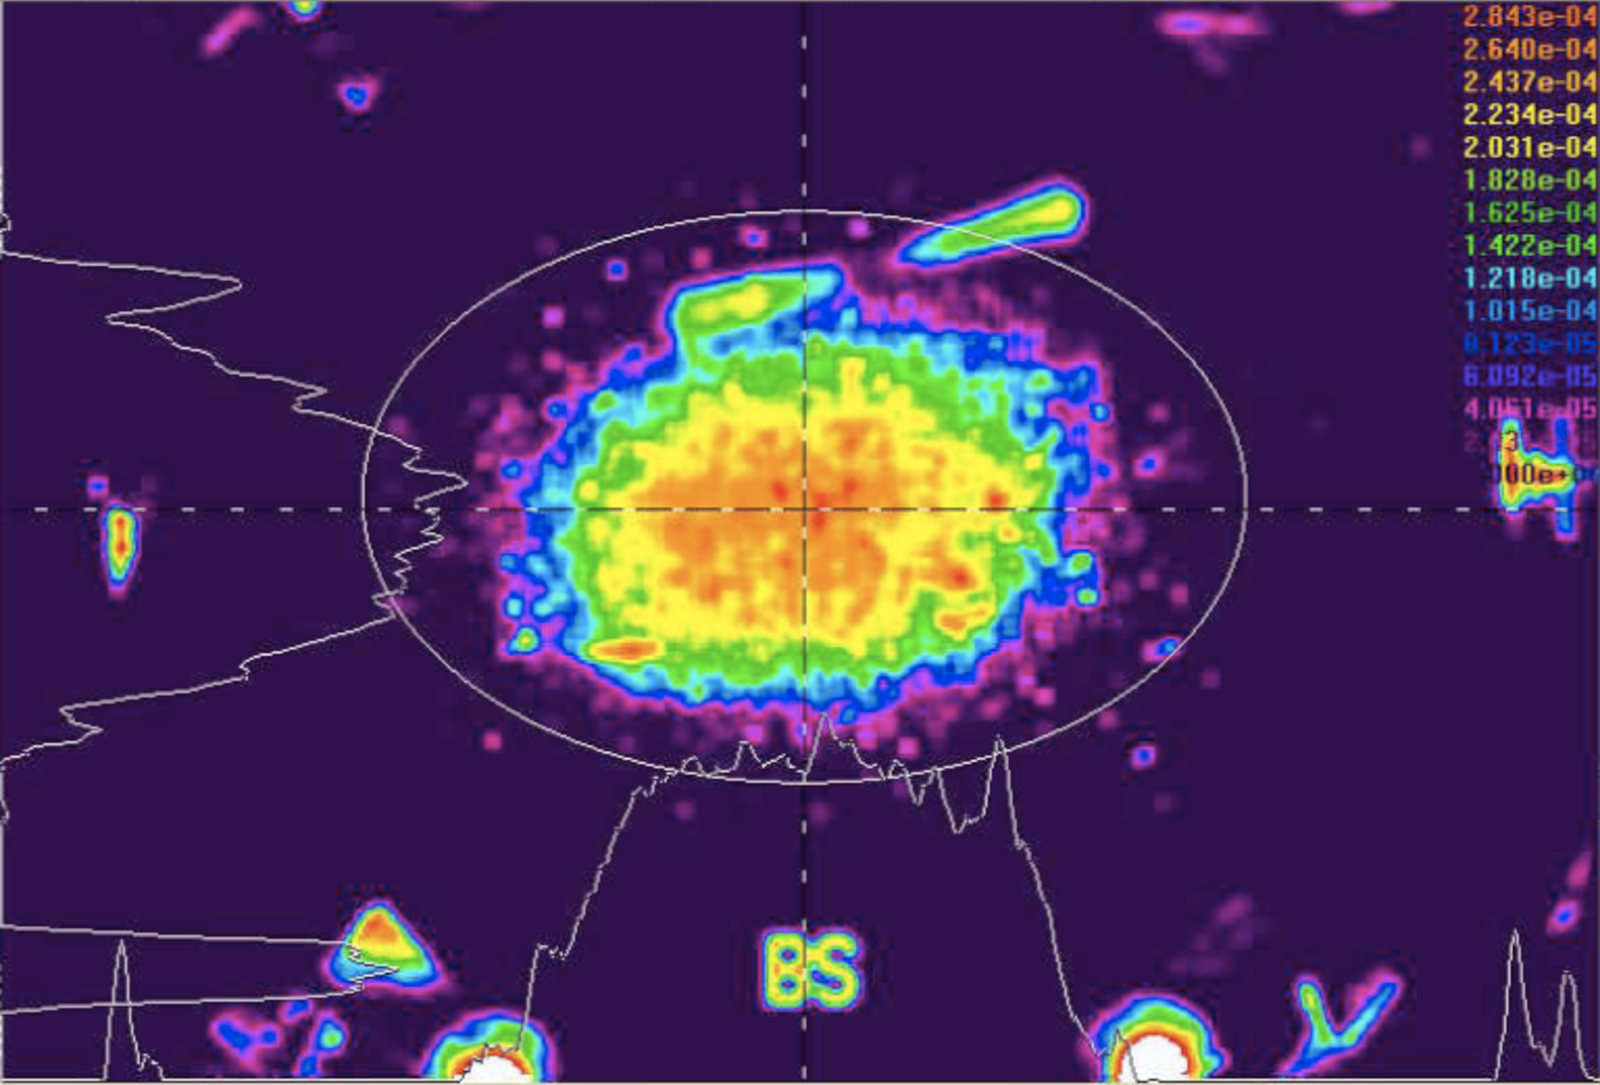
\includegraphics[width=0.8\textwidth]{figures/BCSspiricon.pdf}
% \caption{Image of beam on beam splitter as used for the beam centering servo.}
% \label{fig:BCS}
% \end{centering}
% \end{figure}


% \subsection{QPDs}  
% QPDX and QPDY see the small amount light that is transmitted through
% the ETMs, providing a monitor of the modal axes of the arm cavities. Together with the , they maintain the alignment of the input . QPDX 


% \subsection{WFSs}  
% The wavefront sensors provide the most sophisticated form of
% measuring angular motion of the mirrors. Their frame of reference is
% the fundamental Gaussian mode of the interferometer cavities (x-arm,
% y-arm, recycling cavity) as aligned to ???. All of the mirrors
% globally follow the pointing of the input beam (via the QPDs) which is
% in turn stabilized to the center of the beam splitter (via the BCS) at frequencies well
% below the pendulum resonances. The job of the wavefront sensors is to
% keep the mirrors aligned to one another up to several Hz within this
% hierarchy of alignment. The WFS provide DC and AC control to the
% mirror angles. 




% \section{Control}
% When the gain is really high, comparing the calibrated error and
% control signals shows just what the control loop is doing. The error
% is the residual and the control is what there would be without the
% loop.

% error * (1+G) is the motion without the loop, where G is the open loop gain.

% \begin{itemize} 
% \item optical lever calibration
% \item residuals, perhaps for different kinds of seismic
% \item compare to mirror motion with no ifo (demonstrate ASC suppression)
% \end{itemize}


\begin{figure}
\begin{centering}
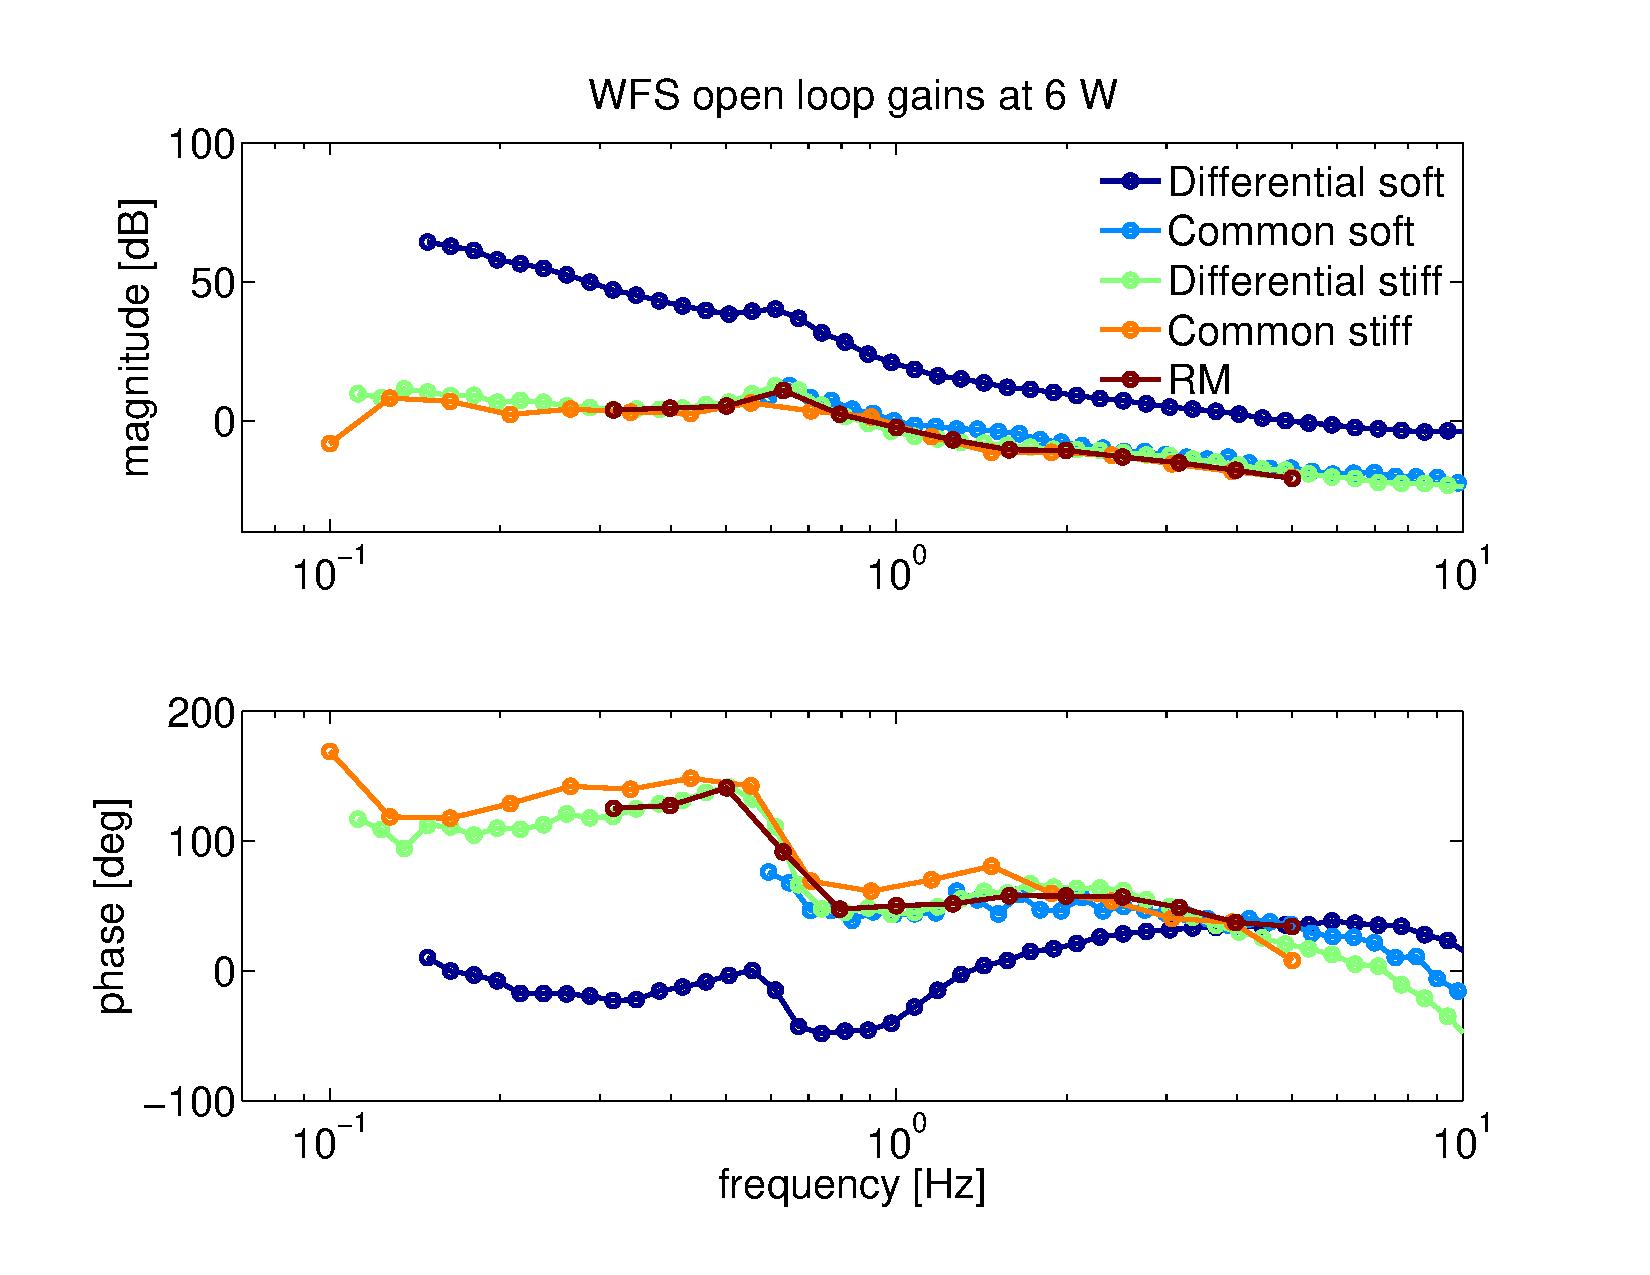
\includegraphics[width=0.8\columnwidth]{figures/olgs6W.pdf}
\caption{Pitch open loop gains of the 5 WFS loops as measured with 6 W
  input power.}
\label{fig:olgs6W}
\end{centering}
\end{figure}



\section{Sensor noise and noise contribution to DARM}


\begin{figure}
\begin{centering}
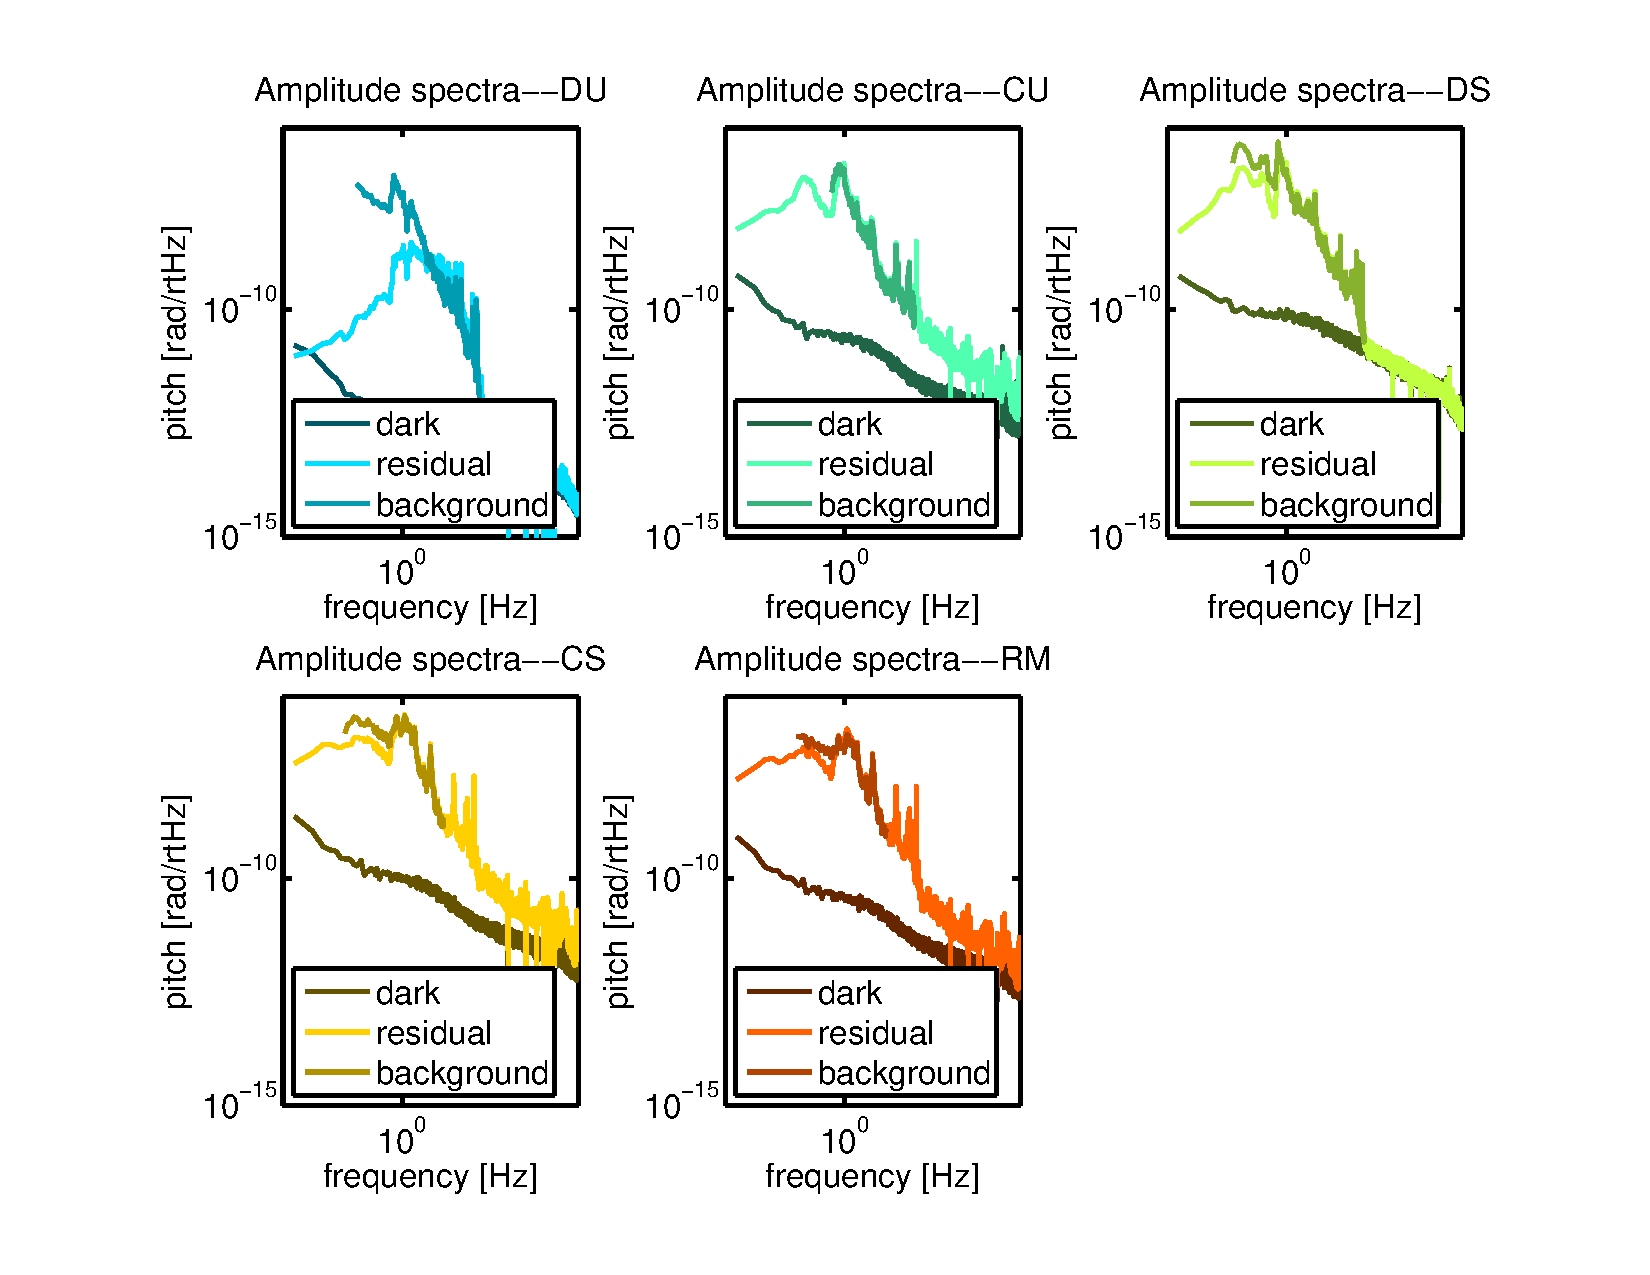
\includegraphics[width=0.7\textwidth]{figures/ASCdofsignals.pdf}
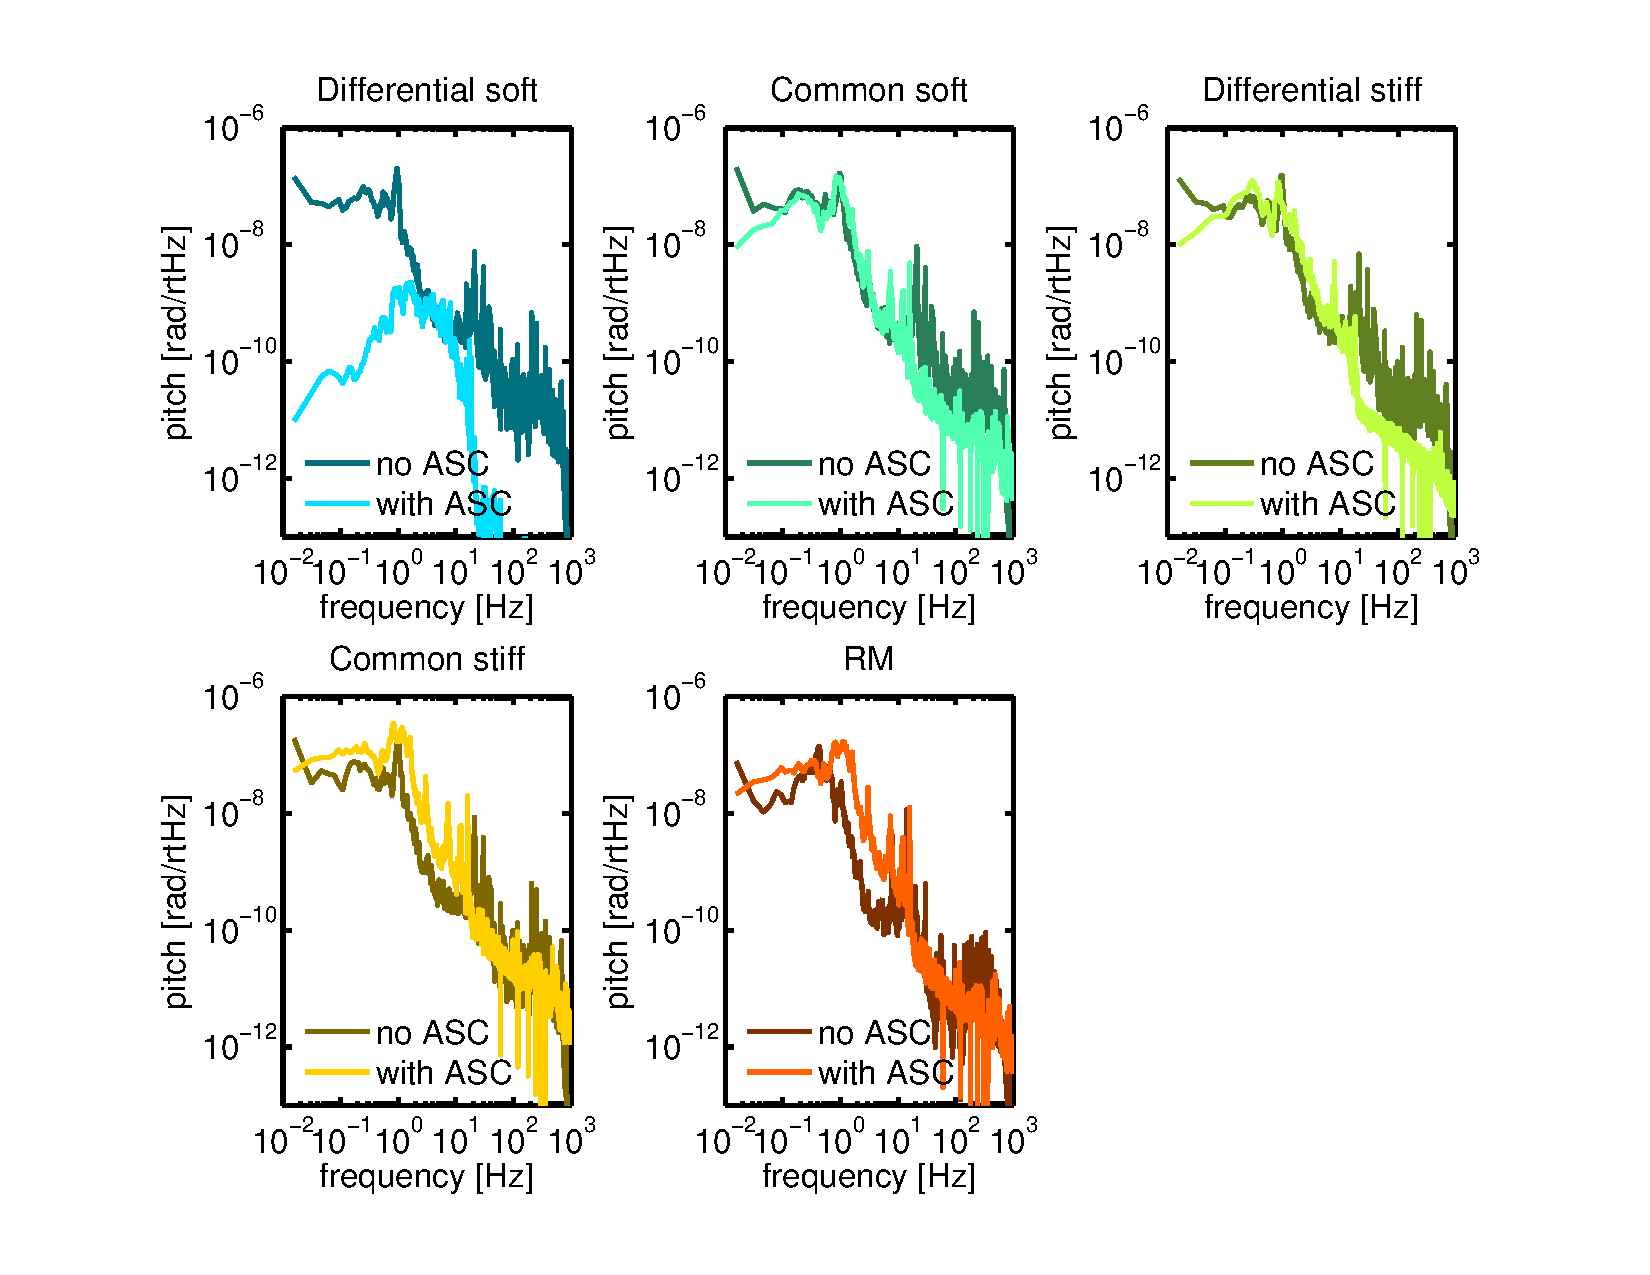
\includegraphics[width=0.7\textwidth]{figures/ASConoff.pdf}
\caption{Top: Comparison of motion with and without the
  ASC. Eigenbasis residual during 10 W lock, and background derived
  from loop correction. Completely different day from bottom
  plot. Bottom: Propagation of sensor signals from 10 W lock through
  input matrix and power scaling to eigenbasis, compared with
  eigenbasis reconstruction of optical lever signals when
  interferometer not locked, but optics under oplev damping. Data are
  taken 45 minutes apart.}
\label{fig:}
\end{centering}
\end{figure}


\section{Solving the noise problem with the eigenbasis}




\section{ASC to DARM noisebudget}
The cut-off frequency of the lowpass filters for the WFS control are
of particular importance in the DARM noisebudget. The lowpass filter
is necessary for suppressing the impression of sensing noise on
suspension control. 

\begin{figure}
\begin{centering}
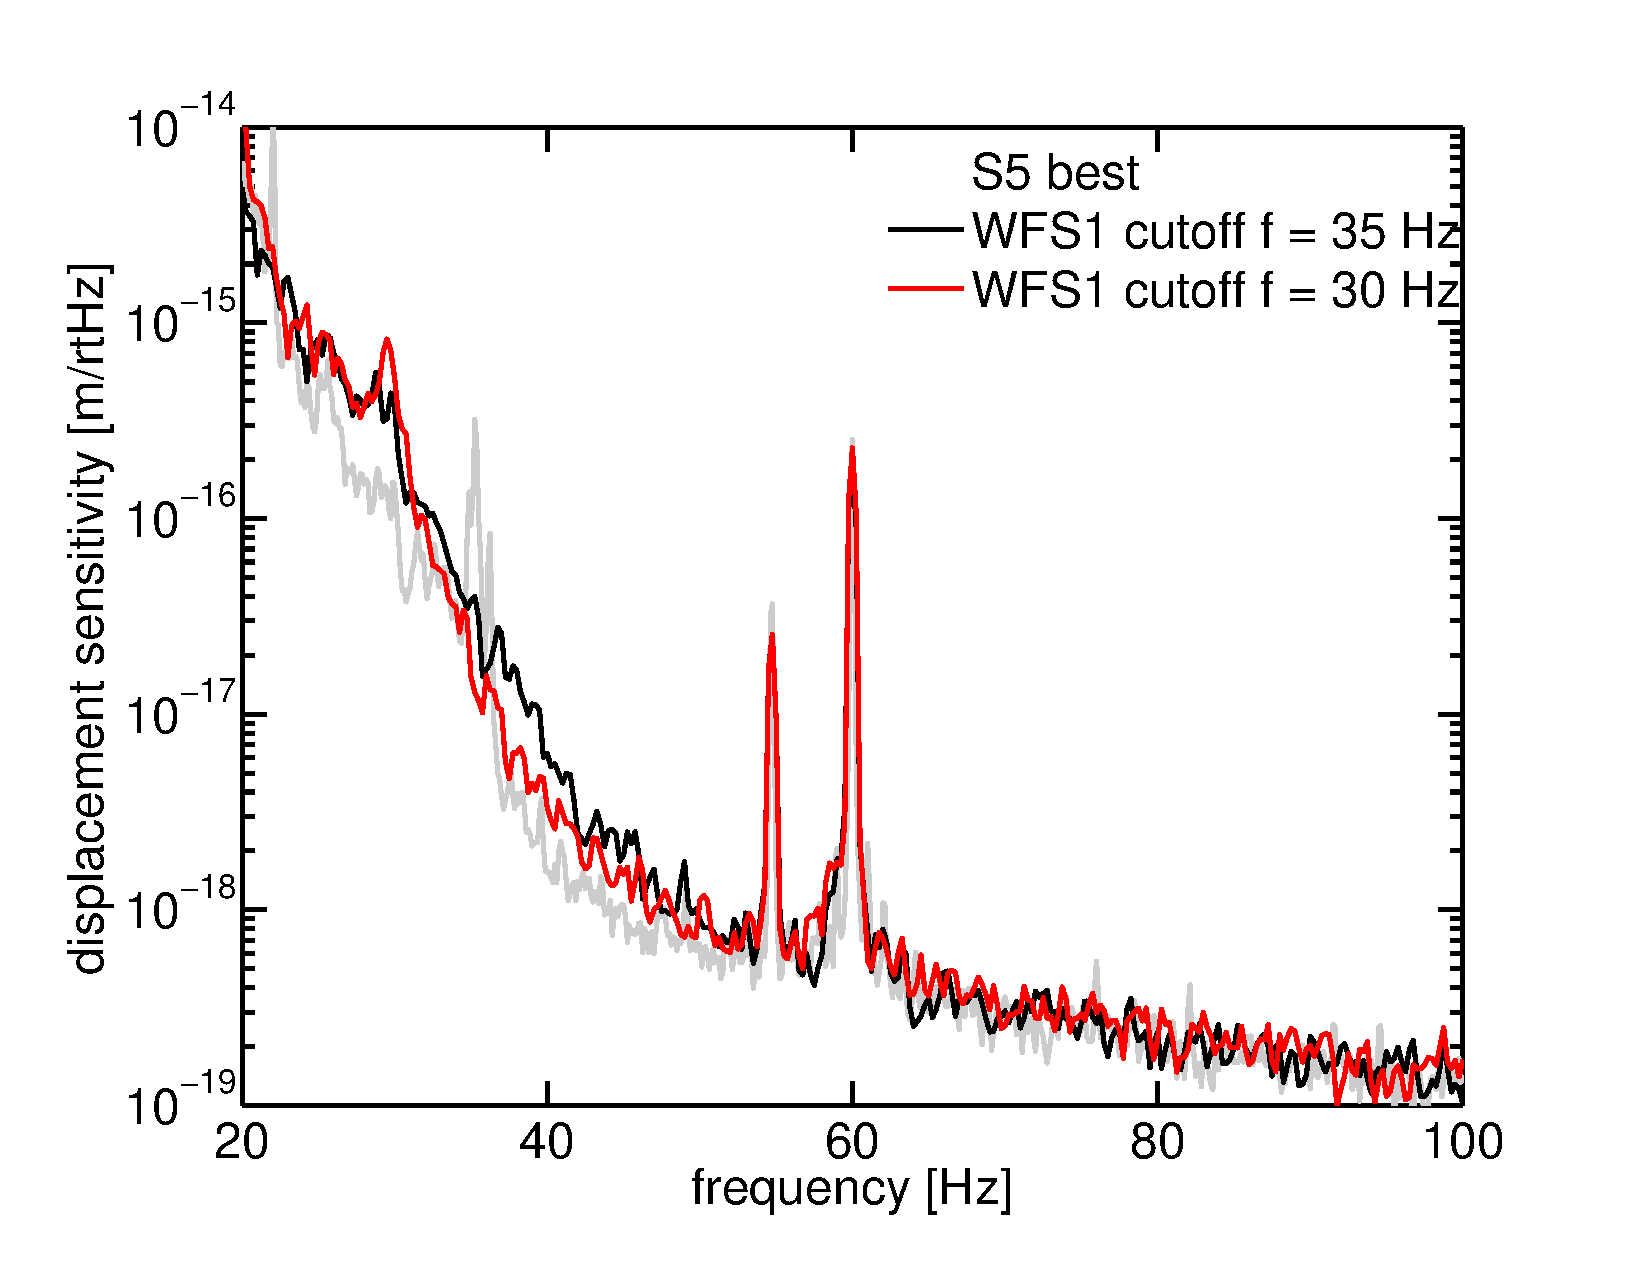
\includegraphics[width=0.8\textwidth]{figures/cutoffWFS1_DARM.pdf}
\caption{Effect of the WFS1 lowpass filter cutoff frequency on strain sensitivity.}
\label{fig:WFS1cutoff}
\end{centering}
\end{figure}







\section{Beam spot motion}
\begin{itemize} 
\item calibration
\item residuals, perhaps for different kinds of seismic
\end{itemize}


\section{Heating related measurements}
\begin{itemize} 
\item effect of PRC g-parameter on ASC sensing matrix
\item SPOB power scaling
\end{itemize}

\section{DC readout related measurements}
\begin{itemize}
\item RF created from DC offset beam moving on WFS1
\item RF vs DC vs power comparison of (AS) beam spot motion on WFS1
\end{itemize}

\section{ASC noisebudget}
\begin{itemize}
\item seismic - breakdown of soure of motion
\item L2A
\item input beam 
\item electronics noise
\item shot noise
\end{itemize}



